\labeledsection{Markov Decision Processes}{sec:mdp}
\centeredtitledbox{Motivation}{
In \linkterm{deterministic}{env_types} environments, the next state is completely determined by the current state and the chosen action. For these problems, we define a corresponding \linkterm{deterministic}{env_types} \linkterm{search problem}{search_problem} where the objective is to find a \linkterm{solution}{search_prob_sol} consisting of a specific \linkterm{sequence}{sequence} of actions—an optimal plan—leading from the initial state to a goal state.

However, in a \linkterm{stochastic}{env_types} environment, the next state is \textbf{not} uniquely determined by the current state and action. In these \linkterm{stochastic}{env_types} \linkterm{search problems}{search_problem}, the \linkterm{agent}{def:agent} controls the action but lacks direct control over the environment's transitions. While the exact outcome of an action is unknown, the \linkterm{agent}{def:agent} knows the probabilities of transitioning to various states given a specific action.

Consequently, a fixed \linkterm{sequence}{sequence} of actions is no longer sufficient. Instead, the goal is to find an \textbf{optimal policy}, $\pi^{*}$, which is a \linkterm{function}{function} $\pi^{*}: \mathcal{S} \to \mathcal{A}$ that dictates the best action for any given state. By following this policy, the \linkterm{agent}{def:agent} navigates the environment's uncertainty to reach a goal state efficiently.
}

\Example{
Consider a grid world where the agent can go west, east, north, or south. Notice the difference between \linkterm{deterministic}{env_types} and \linkterm{stochastic}{env_types} environments:

\begin{figure}[H]
    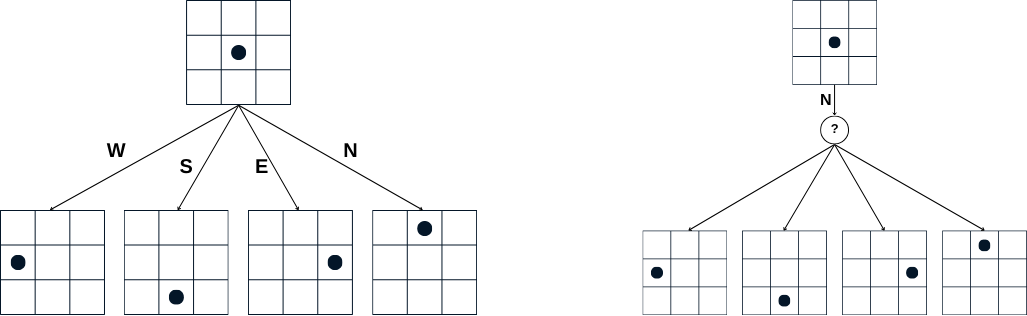
\includegraphics[width=\linewidth]{images/deterministic_vs_stochastic.png}
\end{figure}
}{}

\commandnote{
We are still assuming \linkterm{fully observable}{env_types} environments
}

\definition{MDP Running Example}{
We will consider the following \linkterm{fully observable}{env_types} $4 \times 3$ grid world with \linkterm{stochastic}{env_types} actions:

\begin{figure}[H]
    \centering
    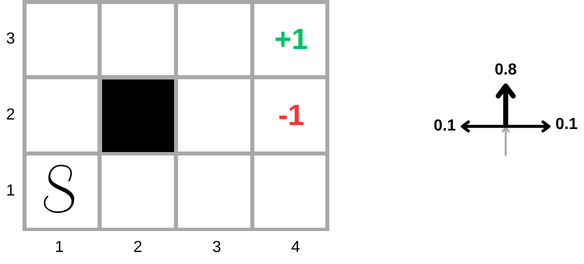
\includegraphics[width=0.4\linewidth]{images/mdp_running_ex.png}
\end{figure}
}{mdp_running_ex}

\definition{MDP}{
A \defemph{Markov Decision Process (MDP)} is the \linkterm{structure}{def:math_structure} $\tuple{\mathcal{S}, \mathcal{A}, \mathcal{T}, \mathcal{I}, R}$ where:
\begin{itemize}
    \item $\mathcal{S}$: the \linkterm{set}{def:set} of states
    \item $\mathcal{I}$: the \linkterm{set}{def:set} of initial states. Since we are in a \linkterm{fully observable}{env_types} environment, $\mathcal{I}=\set{s_0}$.
    \item $\mathcal{A}$: the \linkterm{set}{def:set} of actions, with $\mathcal{A}_s$ denoting the \linkterm{set}{def:set} of action that can be taken from state $s$.
    \item $\mathcal{T}$: a transition model $\mathcal{T}(s,a)=\probd{\mathcal{S}\mid s, a}$
    \item $R$: a \defemph{reward function} $\func{R}{\mathcal{S}}{\mathbb{R}}$ \hfill (we call $R(s)$ a \defemph{reward})
\end{itemize} 
}{MDP}

\ideabox{
We use the \linkterm{rewards}{MDP} as a utility function: the goal is to choose actions such that the expected comulative \linkterm{rewards}{MDP} for the foreseeable future is maximized.
}

\commandnote{
In \linkterm{MDPs}{MDP}, the aim is to find an \textbf{optimal policy} $\pi(s)$, which tells us the best action for every possible state $s$. (because we can't predict where we might end up, we need to consider all states)
}

\definition{Policy}{
A \defemph{policy} $\pi$ for an \linkterm{MDP}{MDP} is a \linkterm{function}{function} mapping each state $s \in \mathcal{S}$ to an action $a \in \mathcal{A}_s$. An \defemph{optimal policy} is a policy that maximizes the expected total \linkterm{rewards}{MDP}.
}{policy}

\Example{
\begin{figure}[H]
     \centering
     \begin{subfigure}[b]{0.24\textwidth}
         \centering
         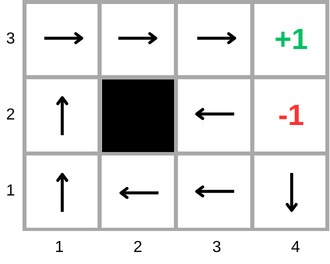
\includegraphics[width=\textwidth]{images/reward-0.01.png}
         \caption{$R(s) = -0.01$}
         \label{fig:sub1}
     \end{subfigure}
     \hfill
     \begin{subfigure}[b]{0.24\textwidth}
         \centering
         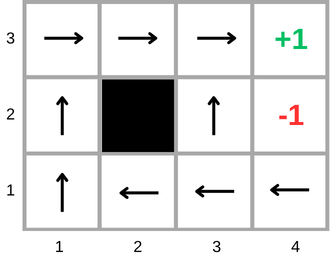
\includegraphics[width=\textwidth]{images/reward-0.03.png}
         \caption{$R(s) = -0.03$}
         \label{fig:sub2}
     \end{subfigure}
     \hfill
     \begin{subfigure}[b]{0.24\textwidth}
         \centering
         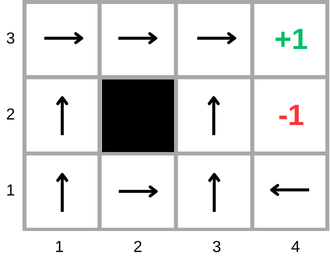
\includegraphics[width=\textwidth]{images/reward-0.4.png}
         \caption{$R(s) = -0.4$}
         \label{fig:sub3}
     \end{subfigure}
     \hfill
     \begin{subfigure}[b]{0.24\textwidth}
         \centering
         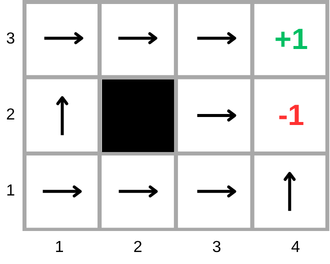
\includegraphics[width=\textwidth]{images/reward-2.png}
         \caption{$R(s) = -2$}
         \label{fig:sub4}
     \end{subfigure}
     \caption{Different optimal policies for different reward functions}
     \label{fig:policy_vs_reward_ex}
\end{figure}

For $R(s) = -0.01$, we have a small negative reward for each state. Hence, each action will cost a little bit and not too much. Therefore, in state $(3,2)$, the optimal action is to go west where there is a $80\%$ chance we stay where we are. We cannot go north since there is a $10\%$ of ending up in the pit ($-1$). Because the action costs only $0.01$, the agent prefers to bang his head to the wall until by chance goes north or south. Similarly, in $(4,1)$.

For $R(s) = -0.03$, the action cost is a bit high. The agent prefer to take the chance of going north (in $(3,2)$) and west in $(4,1)$ regardless of the $10\%$ probability of falling in the pit. 

For $R(s) = -0.4$, the cost now is much higher, the agent will try to finish as soon as possible.

For $R(s) = -2$, life is very painful, the agent might commit suicide to alleviate the pain.
}{}

\noindent\makebox[\textwidth]{%
\rule{0.25\textwidth}{0.4pt}\hfill
\textbf{Exercise : Optimal Policy}\hfill
\rule{0.25\textwidth}{0.4pt}%
}

Give an optimal policy $\pi^{*}$ for the following \linkterm{MDP}{MDP}:
\begin{itemize}
    \item \linkterm{set}{def:set} of states $\mathcal{S} = \set{0,1,2,3,4,5}$ with $\mathcal{I} = \set{0}$
    \item \linkterm{set}{def:set} of actions $\mathcal{A} = \set{-1,1}$
    \item transition model defined as:
    \begin{itemize}
        \item $P((s+a) \mod 6 \mid s,a) = \frac{2}{3}$
        \item $P((s+3) \mod 6 \mid s,a) = \frac{1}{3}$
    \end{itemize}
    \item \linkterm{reward function}{MDP} defined as: $R(5) = 1$ and $R(s) = -0.1 \forall s \in \mathcal{S}\setminus\set{5}$
\end{itemize}

\titledbox{Remember}{
\[
a \bmod b := a - (b \cdot \floor{\frac{a}{b}})
\]
}

\textbf{State $0$}:

\begin{itemize}
    \item $a = -1$
    \begin{itemize}
        \item with prob. $2/3$ we move to $(0 + (-1)) \bmod 6 = 5$
        \item with prob. $1/3$ we move to $(0 + 3) \bmod 6 = 3$
    \end{itemize}
    \item $a = 1$
    \begin{itemize}
        \item with prob. $2/3$ we move to $(0 + 1) \bmod 6 = 1$
        \item with prob. $1/3$ we move to $(0 + 3) \bmod 6 = 3$
    \end{itemize}
\end{itemize}

\redbox{
Optimal action is $a = -1$
}

\textbf{State $1$}:

\begin{itemize}
    \item $a = -1$
    \begin{itemize}
        \item with prob. $2/3$ we move to $(1 + (-1)) \bmod 6 = 0$
        \item with prob. $1/3$ we move to $(1 + 3) \bmod 6 = 4$
    \end{itemize}
    \item $a = 1$
    \begin{itemize}
        \item with prob. $2/3$ we move to $(1 + 1) \bmod 6 = 2$
        \item with prob. $1/3$ we move to $(1 + 3) \bmod 6 = 4$
    \end{itemize}
\end{itemize}

\redbox{
Optimal action is $a = -1$ because with prob. $2/3$ we can go to $0$ and from there we have higher chance to get to $5$.
}

\textbf{State $2$}:

\begin{itemize}
    \item $a = -1$
    \begin{itemize}
        \item with prob. $2/3$ we move to $(2 + (-1)) \bmod 6 = 1$
        \item with prob. $1/3$ we move to $(2 + 3) \bmod 6 = 5$
    \end{itemize}
    \item $a = 1$
    \begin{itemize}
        \item with prob. $2/3$ we move to $(2 + 1) \bmod 6 = 3$
        \item with prob. $1/3$ we move to $(2 + 3) \bmod 6 = 5$
    \end{itemize}
\end{itemize}

\redbox{
No optimal action, same prob. of ending up in $5$, we choose arbitrary
}

\textbf{State $3$}:

\begin{itemize}
    \item $a = -1$
    \begin{itemize}
        \item with prob. $2/3$ we move to $(3 + (-1)) \bmod 6 = 2$
        \item with prob. $1/3$ we move to $(3 + 3) \bmod 6 = 0$
    \end{itemize}
    \item $a = 1$
    \begin{itemize}
        \item with prob. $2/3$ we move to $(3 + 1) \bmod 6 = 4$
        \item with prob. $1/3$ we move to $(3 + 3) \bmod 6 = 0$
    \end{itemize}
\end{itemize}

\redbox{
Optimal action is $a = 1$
}

\textbf{State $4$}:

\begin{itemize}
    \item $a = -1$
    \begin{itemize}
        \item with prob. $2/3$ we move to $(4 + (-1)) \bmod 6 = 3$
        \item with prob. $1/3$ we move to $(4 + 3) \bmod 6 = 1$
    \end{itemize}
    \item $a = 1$
    \begin{itemize}
        \item with prob. $2/3$ we move to $(4 + 1) \bmod 6 = 5$
        \item with prob. $1/3$ we move to $(4 + 3) \bmod 6 = 1$
    \end{itemize}
\end{itemize}

\redbox{
Optimal action is $a = 1$
}

\textbf{State $5$}:

\begin{itemize}
    \item $a = -1$
    \begin{itemize}
        \item with prob. $2/3$ we move to $(5 + (-1)) \bmod 6 = 4$
        \item with prob. $1/3$ we move to $(5 + 3) \bmod 6 = 2$
    \end{itemize}
    \item $a = 1$
    \begin{itemize}
        \item with prob. $2/3$ we move to $(5 + 1) \bmod 6 = 0$
        \item with prob. $1/3$ we move to $(5 + 3) \bmod 6 = 2$
    \end{itemize}
\end{itemize}

\redbox{
No optimal action, we end up in states that have equal rewards, we choose arbitrary
}

Therefore, the optimal policy is:
\begin{itemize}
    \item $\pi^{*}(s) = -1 \quad \forall s \in \set{0,1}$
    \item $\pi^{*}(s) = 1 \quad \forall s \in \set{3,4}$
    \item arbitrary $\quad \forall s \in \set{2,5}$
\end{itemize}
 

\noindent\makebox[\textwidth]{%
\rule{0.3\textwidth}{0.4pt}\hfill
\textbf{End of Exercise}\hfill
\rule{0.3\textwidth}{0.4pt}%
}



\questionbox{
Assume we have two sequences of three actions, the first one will collect the rewards $1,2,2$, and second one will collect $2,3,4$. Which sequence should the agent choose?
}

\answerbox{
Well, since we agreed that we want to maximize the total sum of rewards, obviously we should prefer $2,3,4$ because they sum to $9>5$.
}

\questionbox{
What about $0,0,1$ and $1,0,0$?
}

\observationbox{
They have the same total sum of rewards.
}

\ideabox{
\begin{itemize}
    \item It is reasonable to maximize the sum of rewards
    \item But it is also reasonable to prefer rewards \textbf{now} over rewards \textbf{later}
\end{itemize}
}

\answerbox{
Then the agent should prefer $1,0,0$ over $0,0,1$
}

\questionbox{
But how can we model this into the agent's brain?
}

\answerbox{
We should let the values of the rewards decay exponentially over time
}

\anondefinition{
We call \linkterm{preferences}{preferences} on \linkterm{reward}{MDP} \linkterm{sequences}{sequence} \defemph{stationary} iff
\[
[r, r_0, r_1, r_2, \cdots] \succ [r, r'_0, r'_1, r'_2, \cdots] \Leftrightarrow [r_0, r_1, r_2, \cdots] \succ [r'_0, r'_1, r'_2, \cdots]
\]
}{stationary_preferences}

\Theorem{
For \linkterm{stationary preferences}{stationary_preferences}, there are only two ways to combine \linkterm{rewards}{MDP} over time:
\begin{itemize}
    \item \defemph{additive rewards}: $U([s_0, s_1, s_2, \cdots]) = R(s_0) + R(s_1) + R(s_2) + \cdots$
    \item \defemph{discounted rewards}: $U([s_0, s_1, s_2, \cdots]) = R(s_0) + \gamma R(s_1) + \gamma^2 R(s_2) + \cdots$ where $0 \leq \gamma \leq 1$ is called \defemph{discount factor}
\end{itemize}
}{discounted_rewards}

\questionbox{
Given \linkterm{discounted rewards}{discounted_rewards} with $\gamma=0.5$, what is the utility of the \linkterm{rewards}{MDP} \linkterm{sequences}{sequence} $[1,2,3]$, and $[3,2,1]$?
}

\answerbox{
\begin{itemize}
    \item $U([1,2,3]) = 1 + 0.5 \cdot 2 + 0.25 \cdot 3 = 2.75$
    \item $U([3,2,1]) = 3 + 0.5 \cdot 2 + 0.25 \cdot 1 = 4.25$
\end{itemize}

$U([3,2,1]) >  U([1,2,3])$ (the sooner the better)
}

\minititle{Dicounting Exercise}
Consider the following world:
\begin{figure}[H]
    \centering
    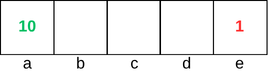
\includegraphics[width=0.2\linewidth]{images/abcde.png}
\end{figure}
\begin{itemize}
    \item $\mathcal{S}=\set{a,b,c,d,e}$
    \item $\mathcal{A}_s = \set{E,W} \quad \forall s \in \set{b,c,d}$ \hfill(East and West)
    \item $\mathcal{T}$ is \linkterm{deterministic}{env_types}
    \item If we are in $a$, we get \linkterm{reward}{MDP} $10$.
    \item If we are in $e$, we get \linkterm{reward}{MDP} $1$.
    \item $R(s)=0 \quad \forall s \in \set{b,c,d}$
\end{itemize}

\questionbox{
For $\gamma=1$ (no \linkterm{discounted rewards}{discounted_rewards}), what is the optimal policy ?
}

\answerbox{
\begin{figure}[H]
    \centering
    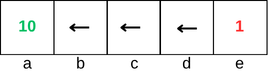
\includegraphics[width=0.2\linewidth]{images/abcde_1.png}
\end{figure}
}

\questionbox{
For $\gamma=0.1$, what is the optimal policy ?
}

\answerbox{
\begin{figure}[H]
    \centering
    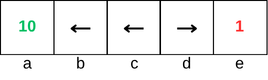
\includegraphics[width=0.2\linewidth]{images/abcde_2.png}
\end{figure}
}

\questionbox{
For which $\gamma$ are West and East equally good when agent in state $d$?
}

\answerbox{
\begin{itemize}
    \item Going East: $0+\gamma \cdot 1$
    \item Going West: $0 + \gamma \cdot 0 + \gamma^2 \cdot 0 + \gamma^3 \cdot 10$
    \item $\gamma = 10 \cdot \gamma^3$
    \item $1 = 10 \cdot \gamma^2$
    \item $\gamma^2 = \frac{1}{10} \leadsto \gamma = \frac{1}{\sqrt{10}}$
\end{itemize}
}

\redbox{
What if we do not have terminal states ?
}

\observationbox{
If we are using \linkterm{additive rewards}{discounted_rewards} and we do not have terminal states, we can get infinite reward!
}

\ideabox{
We have two solutions to this problem:
\begin{itemize}
    \item Finite Horizon: we terminate after a fixed $T$ steps. $\leadsto$ Gives \linkterm{non-stationary}{stationary_preferences} policies ($\pi$ depends on the time left)
    \item Absorbing States: for any policy $\pi$, the agent eventually dies with probability $=1$. $\leadsto$ \linkterm{Expected utility}{expected_utility} of every state is finite
\end{itemize}
}

\observationbox{
A better solution is to use \linkterm{discounted rewards}{discounted_rewards} with $0 \leq \gamma < 1$.
}

\Proof{
\begin{itemize}
\item Let $R_{\text{max}}$ be the maximum reward the agent can get.
\item $U([r_0, r_1, r_2, \cdots, r_{\infty}]) = \sum_{t=0}^{\infty} \gamma^t r_t$
\item $\sum_{t=0}^{\infty} \gamma^t r_t \leq \sum_{t=0}^{\infty} \gamma^t R_{\text{max}}$
\item $\sum_{t=0}^{\infty} \gamma^t R_{\text{max}}$ is a convergent geometric series (since $\gamma < 1$)
\item $\sum_{t=0}^{\infty} \gamma^t R_{\text{max}} = \frac{R_{\text{max}}}{1-\gamma}$
\item Therefore, $U([r_0, r_1, r_2, \cdots, r_{\infty}]) \leq \frac{R_{\text{max}}}{1-\gamma}$
\end{itemize}
}

\minititle{Remember - The Geometric Series}

\anondefinition{
A \textbf{geometric series} is the sum of an infinite sequence where each term is found by multiplying the previous one by a fixed, non-zero constant $r$, called the \textbf{common ratio}. Given an initial term $a \neq 0$, the series is expressed as:
\[ \sum_{n=0}^{\infty} ar^n = a + ar + ar^2 + ar^3 + \dots \]
}{}

To determine if the infinite sum exists, we define the \textbf{$k$-th partial sum}, $S_k$, as the sum of the first $k$ terms:
\[ S_k = \sum_{n=0}^{k-1} ar^n = a + ar + ar^2 + \dots + ar^{k-1} \]
Through algebraic manipulation, this can be written in closed form as:
\[ S_k = a \left( \frac{1-r^k}{1-r} \right) \quad \text{for } r \neq 1 \]


The infinite series converges if the limit of the partial sums exists and is finite:
\[ S = \lim_{k \to \infty} S_k \]

If the magnitude of the ratio is less than one ($|r| < 1$), then the term $r^k$ vanishes as $k$ approaches infinity:
\[ \lim_{k \to \infty} r^k = 0 \]

Substituting this into the partial sum formula yields the \textbf{sum of the infinite geometric series}:
\[ S = \lim_{k \to \infty} a \left( \frac{1-r^k}{1-r} \right) = a \left( \frac{1-0}{1-r} \right) = \frac{a}{1-r} \]

\begin{itemize}
    \item If \textbf{$|r| < 1$}, the series \textbf{converges} to $\frac{a}{1-r}$.
    \item If \textbf{$|r| \geq 1$}, the series \textbf{diverges} (the sum does not approach a finite limit).
\end{itemize}

\anondefinition{
Given a \linkterm{sequence}{sequence} of state $S=s_0, s_1, s_2, \cdots$ and a \linkterm{discount factor}{discounted_rewards} $0 \leq \gamma < 1$, the \defemph{utility} of the \linkterm{sequence}{sequence} is :
\[
U(S) = \sum_{t=0}^{\infty} \gamma^t R(s_t)
\]
}{utility_seq_states_mdp}

\anondefinition{
Given a \linkterm{policy}{policy} $\pi$ and a starting state $s_0$. We define a \linkterm{random variable}{def:random_variable} $S_{s_0}^{\pi}$ which represent the \linkterm{sequence}{sequence} of states resulting from executing $\pi$ at every state starting from $s_0$ (because the environment is \linkterm{stochastic}{env_types}, we do not know the exact sequence, hence the \linkterm{random variable}{def:random_variable} treatment).
}{state_sequence_rv}

\anondefinition{
The \defemph{expected utility} obtained by executing the policy $\pi$ starting in $s_0$ is given by:
\[
U^{\pi} (s_0) := \text{EU}(\linkterm{S_{s_0}^{\pi}}{state_sequence_rv})
\]
}{expected_utility_mdp}

\anondefinition{
The \defemph{optimal policy} $\pi^{*}$ is a policy that maximizes the \linkterm{expected utility}{expected_utility} for the agent:
\[
\pi^{*}_{s_0} := \argmax{\pi} U^{\pi} (s_0)
\]
}{optimal_policy_mdp}

\observationbox{
While we initially define it relative to a starting state $s_0$. It is a fundamental property of MDPs that there exists a single policy $\pi^{*}$ that is optimal for \textbf{all} starting states simultaneously.
}

\anondefinition{
The \defemph{true utility} $U(s)$ of a state is the \linkterm{expected utility}{expected_utility_mdp} obtained by following the \linkterm{optimal policy}{optimal_policy_mdp} starting in that state:
\[ U(s) = U^{\pi^{*}}(s) \]
}{state_utility_mdp}

\anondefinition{
Once these \linkterm{utilities}{state_utility_mdp} are known, the \linkterm{optimal policy}{optimal_policy_mdp} can be extracted locally using the \linkterm{MEU}{def:MEU} principle. Choosing the best action is just maximizing the \linkterm{expected utility}{expected_utility} of the immediate successor states:
\[
\pi^{*}(s) = \argmax{a \in \mathcal{A}_s} \left( \sum_{s'} P(s' \mid s, a) \cdot U(s') \right)
\]
}{optimal_action_mdp}

\redbox{
Given the \linkterm{true utilities}{state_utility_mdp}, we can compute the \linkterm{optimal policy}{optimal_action_mdp} and vice versa.
}

\Example{
Assume we know the \linkterm{utilities}{state_utility_mdp} of our grid world:
\begin{figure}[H]
    \centering
    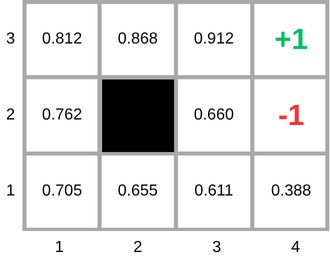
\includegraphics[width=0.3\linewidth]{images/mdp_running_ex_with_utilities.png}
\end{figure}

What is the \linkterm{optimal action}{optimal_action_mdp} for state $(3,4)$?

\begin{align*}
\pi^{*}(s) &= \argmax{a \in \mathcal{A}_s} \left( \sum_{s'} P(s' \mid s, a) \cdot U(s') \right) \\
\pi^{*}((3,4)) &= \argmax{a \in \set{\text{N, S, E, W}}} \left( \sum_{s'} P(s' \mid s, a) \cdot U(s') \right)
\end{align*}

For $a=N$, we have $s' \in \set{(3,2), (4,1), (2,1)}$
\[
\sum_{s'} P(s' \mid s, a) \cdot U(s') = 0.8 \cdot 0.660 + 0.1 \cdot 0.388 + 0.1 \cdot 0.655 = 0.6326
\]

For $a=S$
\[
\sum_{s'} P(s' \mid s, a) \cdot U(s') = 0.8 \cdot 0.611 + 0.1 \cdot 0.388 + 0.1 \cdot 0.655 = 0.5931
\]

For $a=E$
\[
\sum_{s'} P(s' \mid s, a) \cdot U(s') = 0.8 \cdot 0.388 + 0.1 \cdot 0.660 + 0.1 \cdot 0.611 = 0.4375
\]

For $a=W$
\[
\sum_{s'} P(s' \mid s, a) \cdot U(s') = 0.8 \cdot 0.655 + 0.1 \cdot 0.611 + 0.1 \cdot 0.660  = 0.6511
\]

Therefore:
\begin{align*}
\pi^{*}((3,4)) &= \argmax{a \in \set{\text{N, S, E, W}}} \left( \sum_{s'} P(s' \mid s, a) \cdot U(s') \right) = W
\end{align*}
}{}

\questionbox{
How to compute these \linkterm{utilities}{state_utility_mdp} without knowing the \linkterm{optimal policy}{optimal_policy_mdp}?
}

\observationbox{
The expected sum of \linkterm{rewards}{MDP} = current \linkterm{reward}{MDP} + $\gamma \cdot$ expected \linkterm{reward}{MDP} sum after taking the \linkterm{optimal action}{optimal_action_mdp}
}

\centeredtitledbox{Bellman Equation}{
\Theorem{
\[
U(s) := R(s) + \gamma \cdot \max_{a \in \mathcal{A}_s} \sum_{s'} U(s') \cdot P(s' \mid s, a) 
\]
}{bellman_equation}
}

\Example{
Assume our grid world with $R(s)=-0.04$. Then the utility for, e.g. $(1,1)$ is:
\begin{align*}
U(s) &:= R(s) + \gamma \cdot \max_{a \in \mathcal{A}_s} \sum_{s'} U(s') \cdot P(s' \mid s, a) \\
U((1,1)) &:= R((1,1)) + \gamma \cdot \max_{a \in \set{N, S, E, W}} \sum_{s'} U(s') \cdot P(s' \mid (1,1), a) \\
&:= -0.04 + \gamma \cdot \max_{a \in \set{N, S, E, W}} \sum_{s'} U(s') \cdot P(s' \mid (1,1), a) \\[1ex]
% Merged second block
U(1,1) &= -0.04 + \gamma \cdot \max \{ \\
&\quad 0.8U(1,2) + 0.1U(2,1) + 0.1U(1,1), && \textit{North} \\
&\quad 0.9U(1,1) + 0.1U(1,2), && \textit{West} \\
&\quad 0.9U(1,1) + 0.1U(2,1), && \textit{South} \\
&\quad 0.8U(2,1) + 0.1U(1,2) + 0.1U(1,1) \} && \textit{East}
\end{align*}
}{}

\redbox{
\textbf{The Computational Challenge}: The Bellman equations are inherently \textbf{nonlinear} due to the $\max$ operator. This coupling, combined with a high-dimensional state space, renders direct analytical solutions via standard Linear Algebra \textbf{intractable}.
}

\ideabox{
Solve iteratively using e.g., dynamic programming:
\begin{itemize}
    \item Start with arbitrary \linkterm{utility}{state_utility_mdp} values 
    \item At every iteration, update the \linkterm{utility}{state_utility_mdp} values for each state using the values from the previous iteration 
    \item Keep iterating until convergence $\leadsto$ every $s$, eventually will have the true $U(s)$
\end{itemize}
}

\anondefinition{
\centeredtitledbox{Value Iteration}{
\[
U_{i+1}(s) \leftarrow R(s) + \gamma \cdot \max_{a \in \mathcal{A}_s} \sum_{s'} U_i(s') \cdot P(s' \mid s, a) 
\]

\[
\text{Terminate when}\qquad \max_{s \in S} \abs{U_i(s) - U_{i+1}(s)} \qquad \text{is small enough}
\]
}
}{value_iteration}

\anondefinition{
The \textbf{maximum norm} is defined as $\|U\| = \max_{s} |U(s)|$. Consequently, $\|U - V\|$ represents the maximum difference between $U$ and $V$.  
}{maximum_norm}

\Example{
Consider a state space $S = \{s_1, s_2, s_3\}$ with the following utility values:
\[ U = \begin{bmatrix} 2 \\ -5 \\ 4 \end{bmatrix} \]

To find the maximum norm $\|U\|$, we calculate the absolute value for each state and select the largest:
\begin{align*}
\|U\| &= \max_{s \in S} |U(s)| \\
&= \max(\abs{2}, \abs{-5}, \abs{4}) \\
&= \max(2, 5, 4) \\
&= 5
\end{align*}
\redbox{
The maximum norm is $5$ because $-5$ is the value furthest from zero in this vector.
}
}{}

\Example{
Consider two utility vectors $U$ and $V$ for the state space $S = \{s_1, s_2, s_3\}$:
\[ U = \begin{bmatrix} 10 \\ 2 \\ 5 \end{bmatrix}, \quad V = \begin{bmatrix} 7 \\ 2 \\ 8 \end{bmatrix} \]

To find $\|U - V\|$, we find the maximum absolute difference across all states:
\begin{align*}
\|U - V\| &= \max_{s \in S} |U(s) - V(s)| \\
&= \max(|10 - 7|, |2 - 2|, |5 - 8|) \\
&= \max(|3|, |0|, \abs{-3}) \\
&= \max(3, 0, 3) \\
&= 3
\end{align*}

\redbox{
This value represents the largest "error" or shift between the two approximations.
}
}{}

\Theorem{
Let $U^t$ and $U^{t+1}$ be successive approximations to the \linkterm{true utility}{state_utility_mdp} vector $U$ during \linkterm{value iteration}{value_iteration}. Then for any two approximations $U^t$, $V^t$ we have:
\[
\|U^{t+1} - V^{t+1}\| \leq \gamma \|U^{t} - V^{t}\|
\]

where:
\begin{itemize}
    \item $U, V \in \mathbb{R}^{|S|}$ are vectors where each component $U(s)$ represents the expected long-term reward from state $s$.
    \item $\|U - V\|$ is the "distance" between these two utility estimates.
\end{itemize}
$\leadsto$ The update rule ensures that $U$ and $V$ move closer together at a rate defined by the discount factor $\gamma$.
}{thm:contraction_mapping}

\commandnote{
\begin{itemize}
\item That means, any distinct approximations get closer to each other over time. 
\item In our case, they get closer to the \linkterm{true utility}{state_utility_mdp} vector $U$
\item Consequently, \linkterm{value iteration}{value_iteration} converges to a unique, stable, optimal solution 
\end{itemize}
}

\Theorem{
If $\norm{U^{t+1} - U^t} < \epsilon$, then:
\[
\norm{U^{t+1} - U} < \frac{2 \epsilon  \gamma}{1-\gamma} 
\]
}{thm:bellman_error_bound}

\commandnote{
\begin{itemize}
    \item In practice, we cannot check the distance to the \linkterm{true utility}{state_utility_mdp} vector $U$ because it is unknown. We can only check the change between steps: $\|U^{t+1} - U^t\|$.
    \item \Thmref{thm:contraction_mapping} guarantees that if the change in the last step is less than $\epsilon$, then the absolute error from the optimal solution is no larger than $\frac{2\epsilon\gamma}{1-\gamma}$.
    \item As the discount factor $\gamma$ approaches $1$, the denominator $(1-\gamma)$ becomes very small, which makes the error bound much larger. This reflects how "far-sighted" problems are harder to converge.
    \item This allows me to pre-calculate a stopping threshold $\epsilon$ to ensure the final result is within a desired accuracy range.
\end{itemize}
}

\ideabox{
To bridge the gap between theory and code, we use a specific termination condition in the \linkterm{value iteration}{value_iteration} algorithm:
\begin{itemize}
    \item We want the final error to be small, specifically $\|U^{t+1} - U\| < \epsilon$.
    \item During the loop, we track $\delta = \|U^{t+1} - U^t\|$, which is the change between the current and previous guess.
    \item Based on \Thmref{thm:bellman_error_bound}, if we want the true error to be less than $\epsilon$, we must iterate until our observed change $\delta$ satisfies:
    \[
    \delta < \epsilon \frac{(1 - \gamma)}{\gamma}
    \]
    \item As the discount factor $\gamma$ gets closer to 1, the value $(1-\gamma)$ becomes very small. This forces the algorithm to wait until $\delta$ is extremely tiny, ensuring that even small "leftover" changes don't accumulate into a large error over an infinite time horizon.
\end{itemize}
}

\anondefinition{
The \defemph{Value Iteration Algorithm} is given by \Algref{alg:value_iteration}
}{value_iteration_alg}

\begin{algorithm}[H]
\caption{Value Iteration}
\label{alg:value_iteration}
\begin{algorithmic}[1]
\Function{Value-Iteration}{$mdp, \epsilon$}
    \State \textbf{inputs}: $mdp$, an MDP with states $S$, actions $A(s)$, transition model $P(s' \mid s, a)$, rewards $R(s)$, discount $\gamma$
    \State \textbf{inputs}: $\epsilon$, the maximum error allowed in the utility of any state
    \State \textbf{local variables}: $U, U'$, vectors of utilities for states in $S$, initially zero
    \State \textbf{local variables}: $\delta$, the maximum change in the utility of any state in an iteration
    \Repeat
        \State $U \gets U'$
        \State $\delta \gets 0$
        \For{each state $s$ in $S$}
            \State $U'[s] \gets R(s) + \gamma \cdot \max_{a \in A(s)} \sum_{s'} P(s' \mid s, a) U[s']$
            \If{$|U'[s] - U[s]| > \delta$}
                \State $\delta \gets |U'[s] - U[s]|$
            \EndIf
        \EndFor
    \Until{$\delta < \epsilon(1 - \gamma) / \gamma$}
    \State \Return $U$
\EndFunction
\end{algorithmic}
\end{algorithm}

\Example{
Assume again our grid world. We will use $\gamma=1$ (\linkterm{additive rewards}{discounted_rewards}) for simplicity and $R(s)=-0.04$. We start with $U_0(s)=0$, we want to iterate twice to calculate $U_1((3,2))$, $U_1((3,3))$, $U_2((3,2))$ and $U_2((3,3))$:

\begin{figure}[H]
\centering
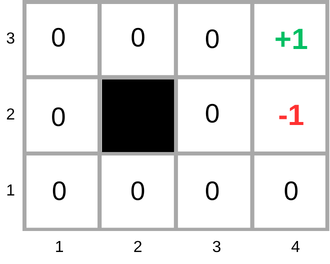
\includegraphics[width=0.3\linewidth]{images/u_0.png}
\caption{$U_0$}
\end{figure}

\begin{align*}
U_{i+1}(s) &\leftarrow R(s) + \gamma \cdot \max_{a} \sum_{s'} U_i(s') \cdot P(s' \mid s, a) \\ 
U_{1}(s_{3,2}) &\leftarrow R(s_{3,2}) + 1 \cdot \max_{a} \sum_{s'} U_0(s') \cdot P(s' \mid s_{3,2}, a) \\ 
U_{1}(s_{3,2}) &\leftarrow -0.04 + 1 \cdot \max_{a} \sum_{s'} U_0(s') \cdot P(s' \mid s_{3,2}, a) \\
&\leftarrow -0.04 + \max \{ \\
&0 \cdot 0.8 + -1 \cdot 0.1 + 0 \cdot 0.1, && \text{North} \\
&-1 \cdot 0.8 + 0 \cdot 0.1 + 0 \cdot 0.1, && \text{East} \\
&0 \cdot 0.8 + 0 \cdot 0.1 + 0 \cdot 0.1, && \text{West} \\
&0 \cdot 0.8 + -1 \cdot 0.1 + 0 \cdot 0.1\} && \text{South} \\
U_{1}(s_{3,2}) &\leftarrow -0.04 + \max \set{-0.1, -0.8, 0, -0.1} \\
U_{1}(s_{3,2}) &\leftarrow -0.04 + 0 \\ 
U_{1}(s_{3,2}) &\leftarrow -0.04
\end{align*}

\begin{align*}
U_{1}(s_{3,3}) &\leftarrow -0.04 + 1 \cdot \max_{a} \sum_{s'} U_0(s') \cdot P(s' \mid s_{3,3}, a) \\
&\leftarrow -0.04 + \max \{ \\
&0 \cdot 0.8 + 1 \cdot 0.1 + 0 \cdot 0.1, && \text{North} \\
&1 \cdot 0.8 + 0 \cdot 0.1 + 0 \cdot 0.1, && \text{East} \\
&0 \cdot 0.8 + 0 \cdot 0.1 + 0 \cdot 0.1, && \text{West} \\
&0 \cdot 0.8 + 1 \cdot 0.1 + 0 \cdot 0.1\} && \text{South} \\
U_{1}(s_{3,3}) &\leftarrow -0.04 + \max \set{0.1, 0.8, 0, 0.1} \\
U_{1}(s_{3,3}) &\leftarrow -0.04 + 0.8 \\ 
U_{1}(s_{3,3}) &\leftarrow 0.76
\end{align*}

\commandnote{
For the first iteration, the only state that will have a positive \linkterm{utility}{state_utility_mdp} is the one that is adjacent to the state where $R(s) = +1$. For every other state, one step will not take us to that state, hence, we will end up having $U(s) = R(s) = -0.04$ for every other state.
}

\begin{figure}[H]
\centering
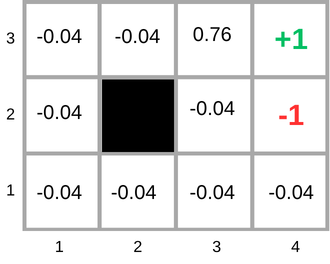
\includegraphics[width=0.3\linewidth]{images/u_1.png}
\caption{$U_1$}
\end{figure}

\redbox{
To generalize, If we are calculating the \linkterm{utility}{state_utility_mdp} estimate for iteration $i$, only the states that can reach the "$+1$" state in $i$ steps or less will have a positive estimate of \linkterm{utility}{state_utility_mdp}.
}

\begin{align*}
U_{i+1}(s) &\leftarrow R(s) + \gamma \cdot \max_{a} \sum_{s'} U_i(s') \cdot P(s' \mid s, a) \\ 
U_{2}(s_{3,2}) &\leftarrow R(s_{3,2}) + 1 \cdot \max_{a} \sum_{s'} U_1(s') \cdot P(s' \mid s_{3,2}, a) \\ 
U_{2}(s_{3,2}) &\leftarrow -0.04 + 1 \cdot \max_{a} \sum_{s'} U_1(s') \cdot P(s' \mid s_{3,2}, a) \\
&\leftarrow -0.04 + \max \{ \\
&0.76 \cdot 0.8 + -1 \cdot 0.1 + -0.04 \cdot 0.1, && \text{North} \\
&-1 \cdot 0.8 + 0.76 \cdot 0.1 + -0.04 \cdot 0.1, && \text{East} \\
&-0.04 \cdot 0.8 + 0.76 \cdot 0.1 + -0.04 \cdot 0.1, && \text{West} \\
&-0.04 \cdot 0.8 + -1 \cdot 0.1 + -0.04 \cdot 0.1\} && \text{South} \\
U_{2}(s_{3,2}) &\leftarrow -0.04 + \max \set{0.504, -0.728, 0.04, -0.136} \\
U_{2}(s_{3,2}) &\leftarrow -0.04 + 0.504 \\ 
U_{2}(s_{3,2}) &\leftarrow 0.464
\end{align*}

\begin{align*}
U_{i+1}(s) &\leftarrow R(s) + \gamma \cdot \max_{a} \sum_{s'} U_i(s') \cdot P(s' \mid s, a) \\ 
U_{2}(s_{3,3}) &\leftarrow R(s_{3,3}) + 1 \cdot \max_{a} \sum_{s'} U_1(s') \cdot P(s' \mid s_{3,3}, a) \\ 
U_{2}(s_{3,3}) &\leftarrow -0.04 + 1 \cdot \max_{a} \sum_{s'} U_1(s') \cdot P(s' \mid s_{3,3}, a) \\
&\leftarrow -0.04 + \max \{ \\
&0.76 \cdot 0.8 + -0.04 \cdot 0.1 + 1 \cdot 0.1, && \text{North} \\
&1 \cdot 0.8 + 0.76 \cdot 0.1 + -0.04 \cdot 0.1, && \text{East} \\
&-0.04 \cdot 0.8 + 0.76 \cdot 0.1 + -0.04 \cdot 0.1, && \text{West} \\
&-0.04 \cdot 0.8 + 1 \cdot 0.1 + -0.04 \cdot 0.1\} && \text{South} \\
U_{2}(s_{3,3}) &\leftarrow -0.04 + \max \set{0.704, 0.872, 0.04, 0.064} \\
U_{2}(s_{3,3}) &\leftarrow -0.04 + 0.872 \\ 
U_{2}(s_{3,3}) &\leftarrow 0.832
\end{align*}

$U_2(s_{2,3})$ will be $0.56$, All other states will have \linkterm{utility}{state_utility_mdp} $=-0.08$. Therefore, second iteration \linkterm{utilities}{state_utility_mdp}:
\begin{figure}[H]
\centering
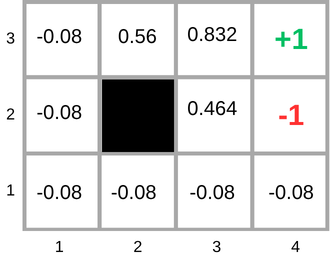
\includegraphics[width=0.3\linewidth]{images/u_2.png}
\caption{$U_2$}
\end{figure}

\redbox{
Again, the states that have positive \linkterm{utilities}{state_utility_mdp} in the second iteration are those which can reach the "$+1$" state in $2$ steps or less.
}
}{}

\observationbox{
While executing the \linkterm{value iteration algorithm}{value_iteration_alg}, you may observe that despite the utility values haven't converged yet, the \linkterm{optimal policy}{optimal_policy_mdp} already stopped changing. 
}

\redbox{
Deriving the \linkterm{optimal policy}{optimal_policy_mdp} doesn't necessarily require us to have accurate estimates of the \linkterm{true utilities}{state_utility_mdp}.
}

\ideabox{
Search for \linkterm{optimal policy}{optimal_policy_mdp} and \linkterm{utility values}{state_utility_mdp} simultaneously $\leadsto$ \textbf{Policy Iteration}
}

\anondefinition{
\defemph{Policy Iteration} alternates between two steps:
\begin{itemize}
    \item \defemph{Policy Evaluation}: Given a \linkterm{policy}{policy} $\pi_i$, calculate $U_i^{\pi}(s)$ which is the \linkterm{utility}{state_utility_mdp} of each state $s$ if $\pi_i$ were to be executed.
    \item \defemph{Policy Improvement}: Calculate a new \linkterm{policy}{policy} $\pi_{i+1}$ using $U_i^{\pi}$
\end{itemize}
Terminate when there is no change in \linkterm{policy}{policy}.
}{policy_iteration}

\titledbox{Value vs Policy Iteration}{
\minititle{Value Iteration:}
\[
U_0(s) \to U_1(s) \to U_2(s) \to \cdots \to U^{*}(s)
\]
Then calculate \linkterm{optimal action}{optimal_action_mdp} for each using:
\[
\pi^{*}(s) = \argmax{a \in \mathcal{A}_s} \left( \sum_{s'} P(s' \mid s, a) \cdot U(s') \right)
\]

\minititle{Policy Iteration:}
\[
\pi_0(s) \quad \overrightarrow{\text{eval}} \quad U_0(s)
\quad \overrightarrow{\text{impr}} \quad
\pi_1(s) \quad \overrightarrow{\text{eval}} \quad U_1(s) 
\cdots 
\pi^{*}(s) \quad \overrightarrow{\text{eval}} \quad U^{*}(s)
\quad \overrightarrow{\text{impr}} \quad
\pi^{*}(s)
\]
}

\centeredtitledbox{Policy Improvement}{
\[
\pi_{i+1}(s) := \argmax{a} \sum_{s'} P(s' \mid a,s) \cdot U_i(s')
\]
}

\centeredtitledbox{Policy Evaluation}{
\[
U_i(s) := R(s) + \gamma \cdot \sum_{s'} P(s' \mid s, \pi_i(s)) \cdot U_i(s')
\]
}

\commandnote{
\begin{itemize}
    \item Notice that we do not have the $\max$ operator anymore since we are already using a policy $\pi_i(s)$.
    \item This yields a linear system of equations where we know everything except the \linkterm{utilities}{state_utility_mdp} (what we solve for)
    \item Solving this system is easier than solving the \linkterm{Bellman Equation}{bellman_equation} where we have a nonlinearity because we do not know the actions ($\max$ operator)
    \item For $n$ states, this will take $\bigo{n^3}$ time.
\end{itemize}
}

\minititle{Policy Iteration Mini Exercise}
\begin{figure}[H]
    \centering
    \begin{minipage}{0.80\textwidth}
        Consider the following grid world with $R(s) = -0.04$ and $\gamma=1$. 
        Assume the initial policy $\pi_0(s_{1,1}) = \pi_0(s_{1,2}) = E$ (east) 
        and the same transition probabilities as before.
    \end{minipage}
    \hfill
    \begin{minipage}{0.1\textwidth}
        \centering
        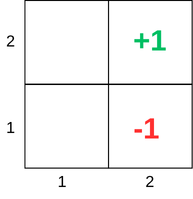
\includegraphics[width=\linewidth]{images/simple_iter.png}
    \end{minipage}
\end{figure}

We evaluate the initial policy:
\begin{align*}
U_i(s) &:= R(s) + \gamma \cdot \sum_{s'} P(s' \mid s, \pi_i(s)) \cdot U_i(s') \\ 
U_0(s) &:= R(s) + \gamma \cdot \sum_{s'} P(s' \mid s, \pi_0(s)) \cdot U_0(s') \\ 
U_0(s_{1,1}) &:= -0.04 + \sum_{s'} P(s' \mid s_{1,1}, E) \cdot U_0(s') \\ 
U_0(s_{1,1}) &:= -0.04 + 0.8 \cdot U_0(s_{2,1}) + 0.1 \cdot U_0(s_{1,2}) + 0.1 \cdot U_0(s_{1,1}) \\ 
U_0(s_{1,1}) &:= -0.04 + 0.8 \cdot -1 + 0.1 \cdot U_0(s_{1,2}) + 0.1 \cdot U_0(s_{1,1}) \\ 
U_0(s_{1,2}) &:= -0.04 + \sum_{s'} P(s' \mid s_{1,2}, E) \cdot U_0(s') \\ 
U_0(s_{1,2}) &:= -0.04 + 0.8 + 0.1 \cdot U_0(s_{1,2}) +  0.1 \cdot U_0(s_{1,1})\\ 
\end{align*}

We have the following system (two equations and two variables):
\begin{align}
    U_0(s_{1,1}) &= -0.84 + 0.1 U_0(s_{1,2}) + 0.1 U_0(s_{1,1}) \label{eq1} \\
    U_0(s_{1,2}) &= 0.76 + 0.1 U_0(s_{1,2}) + 0.1 U_0(s_{1,1}) \label{eq2}
\end{align}

Rearranging terms to the left-hand side:
\begin{align}
    0.9 U_0(s_{1,1}) - 0.1 U_0(s_{1,2}) &= -0.84 \tag{1'} \\
    -0.1 U_0(s_{1,1}) + 0.9 U_0(s_{1,2}) &= 0.76 \tag{2'}
\end{align}

Adding (1') and (2') yields:
\begin{equation*}
    0.8 U_0(s_{1,1}) + 0.8 U_0(s_{1,2}) = -0.08 \implies U_0(s_{1,1}) + U_0(s_{1,2}) = -0.1
\end{equation*}

Solving for $U_0(s_{1,1}) = -0.1 - U_0(s_{1,2})$ and substituting into (2'):
\begin{align*}
    -0.1(-0.1 - U_0(s_{1,2})) + 0.9 U_0(s_{1,2}) &= 0.76 \\
    0.01 + 0.1 U_0(s_{1,2}) + 0.9 U_0(s_{1,2}) &= 0.76 \\
    U_0(s_{1,2}) &= 0.75
\end{align*}

Substituting back to find $U_0(s_{1,1})$:
\begin{equation*}
    U_0(s_{1,1}) = -0.1 - 0.75 = -0.85
\end{equation*}

The final utilities are:
\begin{equation*}
    U_0(s_{1,1}) = -0.85, \quad U_0(s_{1,2}) = 0.75
\end{equation*}

Now we improve:
\begin{align*}
\pi_{i+1}(s) &:= \argmax{a} \sum_{s'} P(s' \mid a,s) \cdot U_i(s') \\
\pi_{1}(s) &:= \argmax{a} \sum_{s'} P(s' \mid a,s) \cdot U_0(s') \\
\pi_{1}(s_{1,1}) &:= \argmax{a} \sum_{s'} P(s' \mid a,s_{1,1}) \cdot U_0(s') \\
\pi_{1}(s_{1,1}) &:= \argmax{a} \{ \\
&0.8 \cdot 0.75 + 0.1 \cdot -1 + 0.1 \cdot -0.85 , && \text{North} \\
&0.8 \cdot -0.85 + 0.1 \cdot -0.85 + 0.1 \cdot -1 ,  && \text{South} \\
&0.8 \cdot -1 + 0.1 \cdot 0.75 + 0.1 \cdot -0.85 ,  && \text{East} \\
&0.8 \cdot -0.85 + 0.1 \cdot 0.75 + 0.1 \cdot -0.85 \} && \text{West} \\
\pi_{1}(s_{1,1}) &:= \argmax{a} \{ \\
&0.415 , && \text{North} \\
&-0.865 ,  && \text{South} \\
&-0.81 ,  && \text{East} \\
&-0.69 \} && \text{West} \\
\pi_{1}(s_{1,1}) &:= N
\end{align*}

Similarly, for $s_{1,2}$:
\begin{align*}
\pi_{1}(s_{1,2}) &:= \argmax{a} \sum_{s'} P(s' \mid a,s_{1,2}) \cdot U_0(s') \\
\pi_{1}(s_{1,2}) &:= \argmax{a} \{ \\
&0.8 \cdot 0.75 + 0.1 \cdot 0.75 + 0.1 \cdot 1 , && \text{North} \\
&0.8 \cdot -0.85 + 0.1 \cdot 0.75 + 0.1 \cdot 1 ,  && \text{South} \\
&0.8 \cdot 1 + 0.1 \cdot 0.75 + 0.1 \cdot -0.85 ,  && \text{East} \\
&0.8 \cdot 0.75 + 0.1 \cdot 0.75 + 0.1 \cdot -0.85 \} && \text{West} \\
\pi_{1}(s_{1,2}) &:= \argmax{a} \{ \\
&0.775 , && \text{North} \\
&-0.505 ,  && \text{South} \\
&0.79 ,  && \text{East} \\
&0.59 \} && \text{West} \\
\pi_{1}(s_{1,2}) &:= E && (\text{didn't change})
\end{align*}

Now we evaluate $\pi_1$:
\begin{align*}
U_i(s) &:= R(s) + \gamma \cdot \sum_{s'} P(s' \mid s, \pi_i(s)) \cdot U_i(s') \\ 
U_1(s) &:= R(s) + \gamma \cdot \sum_{s'} P(s' \mid s, \pi_1(s)) \cdot U_1(s') \\ 
U_1(s_{1,1}) &:= -0.04 + \sum_{s'} P(s' \mid s, \pi_1(s_{1,1})) \cdot U_1(s') \\
U_1(s_{1,1}) &:= -0.04 + 0.8 \cdot U_1(s_{1,2}) + 0.1 \cdot -1 + 0.1 \cdot U_1(s_{1,1}) \\ 
U_1(s_{1,2}) &:= -0.04 + \sum_{s'} P(s' \mid s, \pi_1(s_{1,2})) \cdot U_1(s') \\
U_1(s_{1,2}) &:= -0.04 + 0.8 \cdot 1 + 0.1 \cdot U_1(s_{1,2}) + 0.1 \cdot U_1(s_{1,1}) \\
\end{align*}


We have the following system (two equations and two variables):
\begin{align}
    U_1(s_{1,1}) &:= -0.04 + 0.8 \cdot U_1(s_{1,2}) - 0.1 + 0.1 \cdot U_1(s_{1,1}) \label{eq3} \\
    U_1(s_{1,2}) &:= -0.04 + 0.8 + 0.1 \cdot U_1(s_{1,2}) + 0.1 \cdot U_1(s_{1,1}) \label{eq4}
\end{align}


Rearranging:
\begin{align}
    0.9 U_1(s_{1,1}) - 0.8 U_1(s_{1,2}) &= -0.14 \tag{3'} \\
    -0.1 U_1(s_{1,1}) + 0.9 U_1(s_{1,2}) &= 0.76 \tag{4'}
\end{align}

From (4'), we express $U_1(s_{1,1})$ in terms of $U_1(s_{1,2})$:
\begin{equation*}
    0.1 U_1(s_{1,1}) = 0.9 U_1(s_{1,2}) - 0.76 \implies U_1(s_{1,1}) = 9 U_1(s_{1,2}) - 7.6
\end{equation*}

Substituting this into (3'):
\begin{align*}
    0.9(9 U_1(s_{1,2}) - 7.6) - 0.8 U_1(s_{1,2}) &= -0.14 \\
    8.1 U_1(s_{1,2}) - 6.84 - 0.8 U_1(s_{1,2}) &= -0.14 \\
    7.3 U_1(s_{1,2}) &= 6.7 \\
    U_1(s_{1,2}) &= \frac{67}{73} \approx 0.918
\end{align*}

Substituting back to find $U_1(s_{1,1})$:
\begin{equation*}
    U_1(s_{1,1}) = 9\left(\frac{67}{73}\right) - 7.6 = \frac{603 - 554.8}{73} = \frac{48.2}{73} \approx 0.660
\end{equation*}

The final utilities for $\pi_1$ are:
\begin{equation*}
    U_1(s_{1,1}) \approx 0.660, \quad U_1(s_{1,2}) \approx 0.918
\end{equation*}

Now we improve:
\begin{align*}
\pi_{i+1}(s) &:= \argmax{a} \sum_{s'} P(s' \mid a,s) \cdot U_i(s') \\
\pi_{2}(s) &:= \argmax{a} \sum_{s'} P(s' \mid a,s) \cdot U_1(s') \\
\pi_{2}(s_{1,1}) &:= \argmax{a} \sum_{s'} P(s' \mid a,s_{1,1}) \cdot U_1(s') \\
\pi_{2}(s_{1,1}) &:= \argmax{a} \{ \\
&0.8 \cdot 0.918 + 0.1 \cdot -1 + 0.1 \cdot 0.660 , && \text{North} \\
&0.8 \cdot 0.660 + 0.1 \cdot 0.660 + 0.1 \cdot -1 ,  && \text{South} \\
&0.8 \cdot -1 + 0.1 \cdot 0.918 + 0.1 \cdot 0.660 ,  && \text{East} \\
&0.8 \cdot 0.660 + 0.1 \cdot 0.918 + 0.1 \cdot 0.660 \} && \text{West} \\
\pi_{2}(s_{1,1}) &:= \argmax{a} \{ \\
&0.7004 , && \text{North} \\
&0.494 ,  && \text{South} \\
&-0.6422 ,  && \text{East} \\
&0.6858 \} && \text{West} \\
\pi_{2}(s_{1,1}) &:= N && (\text{didn't change})
\end{align*}

Similarly, for $s_{1,2}$:
\begin{align*}
\pi_{2}(s_{1,2}) &:= \argmax{a} \sum_{s'} P(s' \mid a,s_{1,2}) \cdot U_1(s') \\
\pi_{2}(s_{1,2}) &:= \argmax{a} \{ \\
&0.8 \cdot 0.918 + 0.1 \cdot 0.918 + 0.1 \cdot 1 , && \text{North} \\
&0.8 \cdot 0.660 + 0.1 \cdot 0.918 + 0.1 \cdot 1 ,  && \text{South} \\
&0.8 \cdot 1 + 0.1 \cdot 0.918 + 0.1 \cdot 0.660 ,  && \text{East} \\
&0.8 \cdot 0.918 + 0.1 \cdot 0.918 + 0.1 \cdot 0.660 \} && \text{West} \\
\pi_{2}(s_{1,2}) &:= \argmax{a} \{ \\
&0.9262 , && \text{North} \\
&0.7198 ,  && \text{South} \\
&0.9578 ,  && \text{East} \\
&0.8922 \} && \text{West} \\
\pi_{2}(s_{1,2}) &:= E && (\text{didn't change})
\end{align*}


\begin{figure}[H]
    \centering
    \begin{minipage}{0.80\textwidth}
        \redbox{Since $\pi_1(s) = \pi_2(s) \quad \forall s$, we terminate.}
    \end{minipage}
    \hfill
    \begin{minipage}{0.1\textwidth}
        \centering
        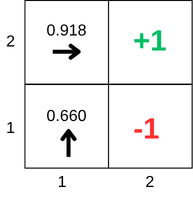
\includegraphics[width=\linewidth]{images/simple_iter_sol.png}
    \end{minipage}
\end{figure}


\newpage
\centeredtitledbox{Motivation}{
So far, we assumed that the environment is \linkterm{fully observable}{env_types}. This means that the \linkterm{agent}{def:agent} always knows exactly which state it is currently in.

However, many environments are only \linkterm{partially observable}{env_types}. In such environments, the \linkterm{agent}{def:agent} cannot directly observe the true state. Instead, it only receives incomplete or noisy information about the state.

To model such situations, we use \defemph{Partially Observable Markov Decision Processes (POMDPs)}.
}

\Example{
Consider an \linkterm{agent}{def:agent} moving on an infinite discrete line. The current position of the \linkterm{agent}{def:agent} is represented by an integer.

The \linkterm{agent}{def:agent} can:
\begin{itemize}
    \item move one step left
    \item move one step right
    \item stay where it is
\end{itemize}

However, actions are stochastic:
\begin{itemize}
    \item moving succeeds only with probability $0.75$
    \item otherwise, the \linkterm{agent}{def:agent} does not move
\end{itemize}

Additionally, the \linkterm{agent}{def:agent} cannot directly observe its exact position. Instead, it receives noisy measurements:
\begin{itemize}
    \item the correct position is measured with probability $0.5$
    \item a neighboring position is measured with probability $0.25$
\end{itemize}
}{}

\definition{POMDP}{
A \defemph{Partially Observable Markov Decision Process (POMDP)} is the structure
\[
\tuple{\mathcal{S},\mathcal{A},\mathcal{T},\mathcal{I},R,\mathcal{E},O}
\]
where:
\begin{itemize}
    \item $\mathcal{S}$ is the set of states
    \item $\mathcal{A}$ is the set of actions
    \item $\mathcal{T}$ is the transition model $\mathcal{T}(s,a)=\probd{\mathcal{S}\mid s,a}$
    \item $\mathcal{I}$ is the initial probability distribution over states
    \item $\func{R}{\mathcal{S}}{\mathbb{R}}$ is the reward function
    \item $\mathcal{E}$ is the set of possible observations
    \item $O$ is the observation model such that $O(s,e)=P(e\mid s)$
\end{itemize}
}{pomdp}

\Example{
For our line-navigation problem:
\[
\mathcal{S}=\mathbb{Z}
\]

The actions are:
\[
\mathcal{A}=\set{-1,0,+1}
\]

Example initial probability distribution:
\[
\mathcal{I}=\set{(4,0.6),(5,0.4)}
\]

This means the \linkterm{agent}{def:agent} initially believes:
\begin{itemize}
    \item it is in position $4$ with probability $0.6$
    \item it is in position $5$ with probability $0.4$
\end{itemize}
}{}

\observationbox{
Compared to an \linkterm{MDP}{MDP}, a \linkterm{POMDP}{pomdp} introduces an additional source of uncertainty:
\begin{itemize}
    \item in an \linkterm{MDP}{MDP}, the current state is known exactly
    \item in a \linkterm{POMDP}{pomdp}, the \linkterm{agent}{def:agent} only receives observations about the state
\end{itemize}
}

\definition{Belief State}{
A \defemph{belief state} is a probability distribution over states:
\[
b=\probd{\mathcal{S}}
\]
where $b(s)$ denotes the probability assigned to state $s$.
}{belief_state}

\ideabox{
In a \linkterm{POMDP}{pomdp}, the \linkterm{agent}{def:agent} does not know the true current state.

Therefore, instead of storing a single state, it stores a probability distribution over all possible states.

This distribution is called the \linkterm{belief state}{belief_state}.
}

\definition{POMDP Decision Cycle}{
A \linkterm{POMDP}{pomdp} proceeds in the following cycle:
\begin{enumerate}
    \item the \linkterm{agent}{def:agent} starts with a \linkterm{belief state}{belief_state}
    \item the \linkterm{agent}{def:agent} executes an action
    \item the environment changes according to the transition model
    \item the \linkterm{agent}{def:agent} receives an observation
    \item the \linkterm{agent}{def:agent} updates its \linkterm{belief state}{belief_state}
\end{enumerate}
}{pomdp_cycle}

\Example{
Suppose the \linkterm{agent}{def:agent} currently has:
\[
b_0=\set{(4,0.6),(5,0.4)}
\]

and executes action $+1$.

The \linkterm{agent}{def:agent} then:
\begin{enumerate}
    \item computes the new probabilities after the stochastic movement
    \item receives a noisy observation
    \item updates the belief state using the observation
\end{enumerate}
}{}

\definition{Transition Model in a POMDP}{
The \defemph{transition model} describes how actions probabilistically change the state:
\[
\mathcal{T}(s,a)=\probd{\mathcal{S}\mid s,a}
\]
}{pomdp_transition_model}

\Example{
For action $+1$:
\[
\mathcal{T}(n,+1)
=
\set{
(n+1,0.75),
(n,0.25)
}
\]

This means:
\begin{itemize}
    \item with probability $0.75$, the \linkterm{agent}{def:agent} successfully moves right
    \item with probability $0.25$, it stays where it is
\end{itemize}

Similarly:
\[
\mathcal{T}(n,-1)
=
\set{
(n-1,0.75),
(n,0.25)
}
\]
}{}

\definition{Observation Model}{
The \defemph{observation model} specifies the probability of receiving observation $e$ while being in state $s$:
\[
O(s,e)=P(e\mid s)
\]
}{observation_model}

\Example{
\[
O
=
\set{
(s,s-1,0.25),
(s,s,0.5),
(s,s+1,0.25)
}
\]

This means:
\begin{itemize}
    \item if the agent observes it is in $s$, there is a $0.5$ chance it is actually there,
    \item and there is a $0.25$ chance it is at $s-1$, and another $0.25$ chance it is at $s+1$.
\end{itemize}
}{}

\minititle{Belief State Update}

Assume the current belief state is:
\[
b_0=\set{(4,0.6),(5,0.4)}
\]

The \linkterm{agent}{def:agent} executes action $+1$.

Recall:
\[
\mathcal{T}(n,+1)
=
\set{
(n+1,0.75),
(n,0.25)
}
\]

We now compute the probability for each possible successor state separately.


\textbf{State $4$}

The only way to end in state $4$ is:
\begin{itemize}
    \item start in state $4$
    \item fail to move
\end{itemize}

Thus:
\[
b_a(4)
=
0.6\cdot 0.25
=
0.15
\]

\textbf{State $5$}

There are two ways to end in state $5$:
\begin{itemize}
    \item start in state $4$ and successfully move right
    \item start in state $5$ and fail to move
\end{itemize}

Thus:
\[
b_a(5)
=
0.6\cdot 0.75
+
0.4\cdot 0.25
=
0.45+0.10
=
0.55
\]

\textbf{State $6$}

The only way to end in state $6$ is:
\begin{itemize}
    \item start in state $5$
    \item successfully move right
\end{itemize}

Thus:
\[
b_a(6)
=
0.4\cdot 0.75
=
0.3
\]

Therefore, the resulting \linkterm{belief state}{belief_state} is:
\[
b_a
=
\set{
(4,0.15),
(5,0.55),
(6,0.3)
}
\]

Suppose the \linkterm{agent}{def:agent} now observes position $4$.

Recall that the predicted \linkterm{belief state}{belief_state} after executing action $+1$ was:
\[
b_a
=
\set{
(4,0.15),
(5,0.55),
(6,0.3)
}
\]

This means:
\begin{itemize}
    \item the \linkterm{agent}{def:agent} believes it is in state $4$ with probability $0.15$
    \item in state $5$ with probability $0.55$
    \item in state $6$ with probability $0.3$
\end{itemize}

Now the \linkterm{agent}{def:agent} receives the observation $4$.

We use the observation model:
\[
O
=
\set{
(s,s-1,0.25),
(s,s,0.5),
(s,s+1,0.25)
}
\]

We now ask:

\begin{quote}
How likely is it to observe $4$ from each possible state?
\end{quote}

\paragraph{Case 1: True state is $4$}

If the true state is $4$, then observing $4$ is correct.

Thus:
\[
O(4,4)=0.5
\]

The prior probability of being in state $4$ was:
\[
b_a(4)=0.15
\]

Therefore:
\[
P(4,4)
=
b_a(4)\cdot O(4,4)
=
0.15\cdot 0.5
=
0.075
\]

\paragraph{Case 2: True state is $5$}

If the true state is $5$, then observing $4$ means measuring one step too far left.

Thus:
\[
O(5,4)=0.25
\]

The prior probability of being in state $5$ was:
\[
b_a(5)=0.55
\]

Therefore:
\[
P(5,4)
=
b_a(5)\cdot O(5,4)
=
0.55\cdot 0.25
=
0.1375
\]

\paragraph{Case 3: True state is $6$}

If the true state is $6$, then observing $4$ would require an error of two positions.

This is impossible in our observation model.

Thus:
\[
O(6,4)=0
\]

Therefore:
\[
P(6,4)
=
b_a(6)\cdot O(6,4)
=
0.3\cdot 0
=
0
\]

Combining all values yields the unnormalized updated belief state:
\[
\set{
(4,0.075),
(5,0.1375)
}
\]

However, this is not yet a probability distribution, because the probabilities do not sum to $1$:
\[
0.075+0.1375=0.2125
\]

Therefore, we normalize the values.

\paragraph{Normalized probability for state $4$}

\[
b'(4)
=
\frac{0.075}{0.2125}
\approx
0.35
\]

\paragraph{Normalized probability for state $5$}

\[
b'(5)
=
\frac{0.1375}{0.2125}
\approx
0.65
\]

Thus, the updated \linkterm{belief state}{belief_state} becomes:
\[
b'
\approx
\set{
(4,0.35),
(5,0.65)
}
\]

\ideabox{
Observation $4$ increases the probability of state $5$ more strongly than state $4$ because state $5$ already had a much larger prior probability before the observation.
}


\definition{Belief-State MDP}{
Every \linkterm{POMDP}{pomdp} can be transformed into an equivalent \linkterm{MDP}{MDP} whose states are \linkterm{belief states}{belief_state}.
}{belief_mdp}

\observationbox{
In the transformed \linkterm{MDP}{MDP}:
\begin{itemize}
    \item a state is no longer a concrete world state
    \item instead, a state is a probability distribution over world states
\end{itemize}
}


\definition{Reward Function on Belief States}{
The reward of a \linkterm{belief state}{belief_state} is defined as its expected reward:
\[
R'(b)
=
\sum_{s\in\mathcal{S}}
R(s)\cdot b(s)
\]
}{belief_reward}

\Example{
Suppose:
\[
R(0)=1
\]
and:
\[
R(s)=-0.1
\qquad
\text{for all } s\neq 0
\]

For:
\[
b
=
\set{
(4,0.15),
(5,0.55),
(6,0.3)
}
\]

we obtain:
\[
R'(b)
=
(-0.1)\cdot 0.15
+
(-0.1)\cdot 0.55
+
(-0.1)\cdot 0.3
=
-0.1
\]
}{}

\redbox{
Although \linkterm{POMDPs}{pomdp} can be reduced to \linkterm{belief-state MDPs}{belief_mdp}, solving them exactly is computationally very difficult.
}

\Theorem{
Solving finite-horizon \linkterm{POMDPs}{pomdp} is PSPACE-hard.
}{}

\commandnote{
The difficulty comes from the fact that the \linkterm{belief-state space}{belief_state} is typically infinite. Even if the original state space is finite, there are infinitely many possible probability distributions over it.
}
